
%(BEGIN_QUESTION)
% Copyright 2010, Tony R. Kuphaldt, released under the Creative Commons Attribution License (v 1.0)
% This means you may do almost anything with this work of mine, so long as you give me proper credit

Calculate the output voltage rate-of-change (volts per second) of this controller circuit if the PV signal is 3.0 volts and the SP signal is 2.5 volts, assuming the potentiometer is set for maximum resistance.  Also calculate the ``time constant'' value of $\tau$ for this circuit at this same potentiometer position:

$$\includegraphics[width=15.5cm]{i01589x01.eps}$$

Next, calculate the amount of time it takes for the output to change by 0.5 volts (the same amount as the difference between PV and SP) when the potentiometer is exactly at the half-way position.  How does this time figure compare with the new value for $\tau$ at this pot position?

\vskip 20pt \vbox{\hrule \hbox{\strut \vrule{} {\bf Suggestions for Socratic discussion} \vrule} \hrule}

\begin{itemize}
\item{} Identify a way to shorten the integration time constant of this controller without adjusting the 71 k$\Omega$ potentiometer located in module 4.
\item{} Identify a way to shorten the integration time constant without changing anything at all in module 4.
\item{} Identify the action (direct or reverse) of this controller, and then identify what you would have to alter in the circuit to reverse that action.
\end{itemize}

\underbar{file i01589}
%(END_QUESTION)





%(BEGIN_ANSWER)

$d\hbox{(Output)} \over dt$ = $-149.8$ mV/s with 0.5 volt error and maximum resistance.

\vskip 10pt

$\tau_i$ = 3.337 seconds per repeat (3.337 seconds to ``repeat'' the 0.5 volt error signal) when the pot is set for maximum resistance.

\vskip 10pt

$\tau_i$ = 1.669 seconds per repeat (1.669 seconds to ``repeat'' the 0.5 volt error signal) when the pot is set for 35.5 k$\Omega$.

%(END_ANSWER)





%(BEGIN_NOTES)

This integrator circuit basically executes the following mathematical function:

$$V_{out} = - {1 \over RC} \int_0^T (\hbox{PV} - \hbox{SP}) \> dt$$

Plugging in the given values for the maximum-resistance scenario:

$$V_{out} = - {1 \over (71000)(0.000047)} \int_0^T (3 - 2.5) \> dt$$

If we let this circuit integrate for 1 seconds' worth of time, we get:

$$V_{out} = - {1 \over (71000)(0.000047)} \int_0^1 (3 - 2.5) \> dt$$

$$V_{out} = - {1 \over 3.337} \int_0^1 0.5 \> dt$$

$$V_{out} = - \left({1 \over 3.337}\right) [(1)(0.5) - (0)(0.5)]$$

$$V_{out} = - \left({1 \over 3.337}\right) (0.5)$$

$$V_{out} = - 0.149835 \hbox{ volts}$$

The integration time constant ($\tau_i$) is the product of $R$ and $C$, which in the maximum-resistance scenario is 3.337 seconds.

\vskip 10pt

If we set the potentiometer at its half-way position, $R$ will be 35.5 k$\Omega$ and the integration time constant will be half of its full value (1.6685 seconds).  If we run another ``thought experiment'' to let the integrator circuit do it's thing for exactly one second, we get this result:

$$V_{out} = - {1 \over (35500)(0.000047)} \int_0^1 (3 - 2.5) \> dt$$

$$V_{out} = - {1 \over 1.6685} \int_0^1 0.5 \> dt$$

$$V_{out} = - \left({1 \over 1.6685}\right) [(1)(0.5) - (0)(0.5)]$$

$$V_{out} = - \left({1 \over 1.6685}\right) (0.5)$$

$$V_{out} = - 0.29967 \hbox{ volts}$$

Given a constant error between PV and SP, the integrator's output voltage will be a linear ramp.  Therefore, we can regard the output voltage at 1 second as the rate-of-change of that voltage in volts per second (assuming in both cases the integrator's output began at 0 volts).  To solve for the amount of time required for a ramping voltage of $-0.29967$ volts per second to reach $-0.5$ volts, all we need to do is divide the two figures to cancel out volts and leave us with seconds:

$${-0.5 \hbox{ V} \over -0.29967 \hbox{ V/s}} = 1.6685 \hbox{ s}$$

Thus, we see that the definition of ``time constant'' ($\tau$) for an integrator is the amount of time it takes to ``repeat'' the input signal.

%INDEX% Control, integral: analog electronic controller

%(END_NOTES)


